\begin{figure}[H]
\centering
\begin{annotatedFigure}
	{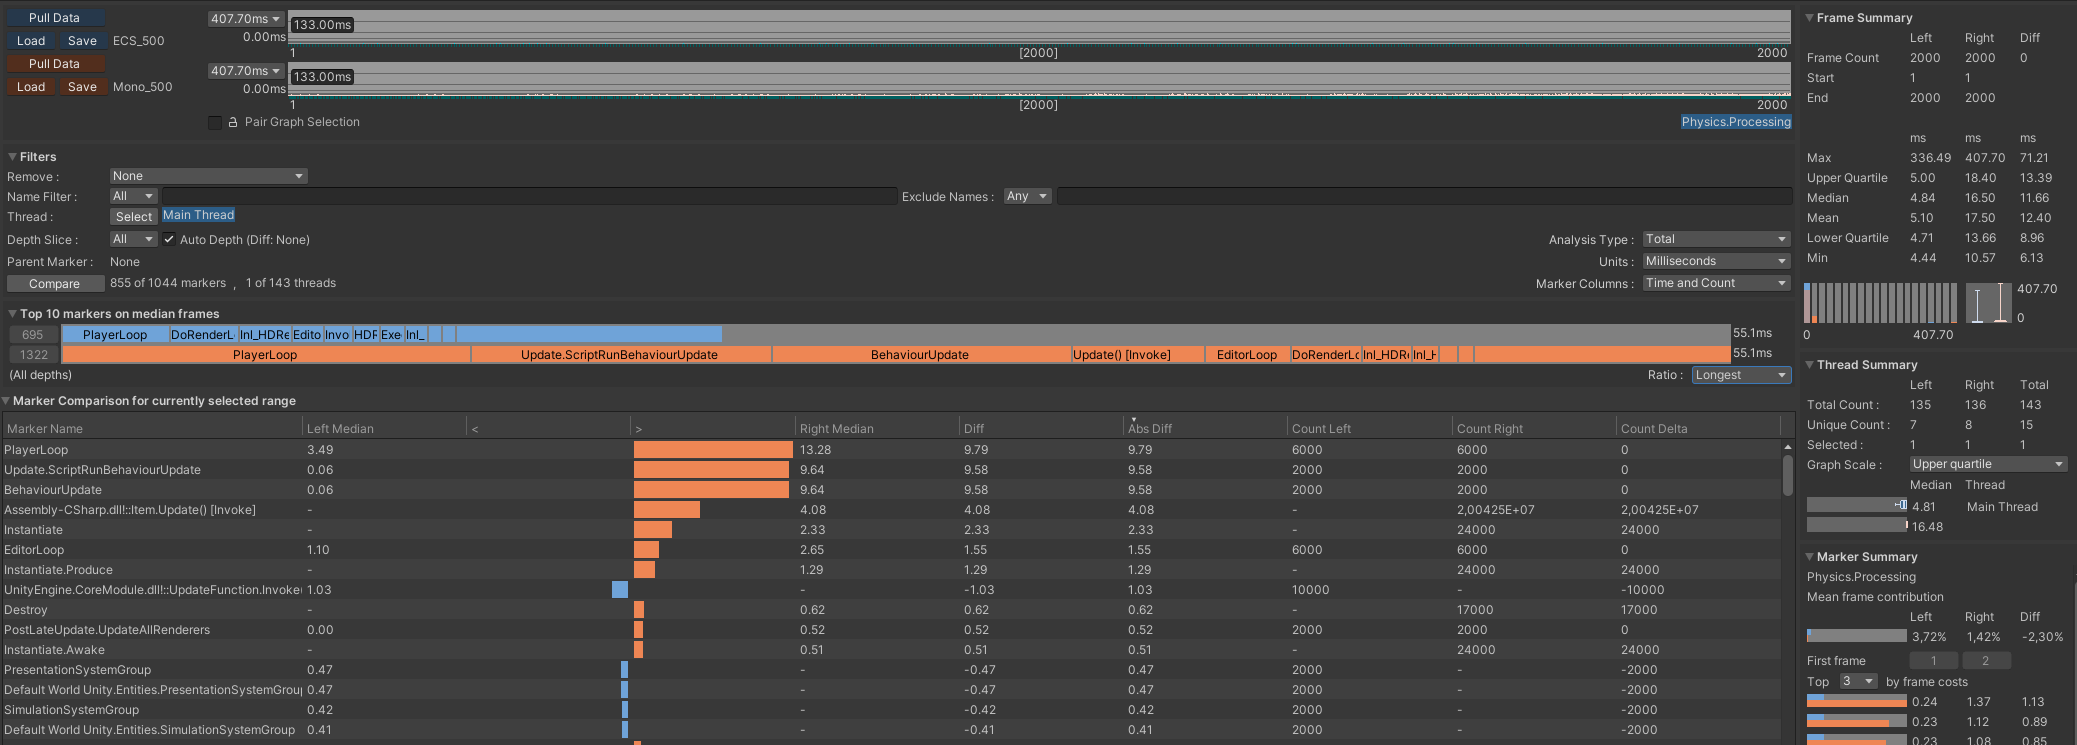
\includegraphics[scale=0.31]{Bilder/Profile Analyzer.png}}
	\annotatedFigureBox{-0.005,0.8046}{0.182,1.01}{A}{0.182,0.8046}
	\annotatedFigureBox{0.86,-0.01}{1.005,1.01}{D}{1.005,-0.01}
	\annotatedFigureBox{-0.005,0.4842}{0.857,0.5942}{B}{0.857,0.4842}
	\annotatedFigureBox{-0.005,-0.01}{0.445,0.4804}{C}{0.445,-0.01}
\end{annotatedFigure}
\caption[Der \textit{Profile Analyzer} im Unity Editor]{Der \textit{Profile Analyzer} im Unity Editor. Es werden die Mono- und die \textit{ECS} Messdaten des Spiels miteinander verglichen. Links oben (A) erkennt man, welche Daten man gerade vergleicht und sieht dazu eine Timeline beider Daten. Die \textit{ECS} Daten sind im Bild blau dargestellt, die Mono Daten rot. In der Mitte des Bildes (B) hat man den Vergleich des Median Bildes. Deutlich zu erkennen ist die wesentlich kürzere Laufzeit des \textit{ECS} Bildes. In dem unteren Teil (C) werden wichtige Spielfunktionen im Vergleich dargestellt. Beispielsweise ist ganz oben der \textit{PlayerLoop} (gesamte Berechnungszeit eines Bildes). Dazu erkennt man an dem Balken, welches der Spiele eine höhere Berechnungszeit hatte. Rechts (D) gibt es zusätzlich noch eine Zusammenfassung über die gesamte Anzahl an Bildern und Threads in beiden Spielen.}
\label{fig:profile_analyzer}
\end{figure}